% Redistribution probes flow
\documentclass[tikz,border=5pt]{standalone}
\usetikzlibrary{arrows.meta}
\begin{document}
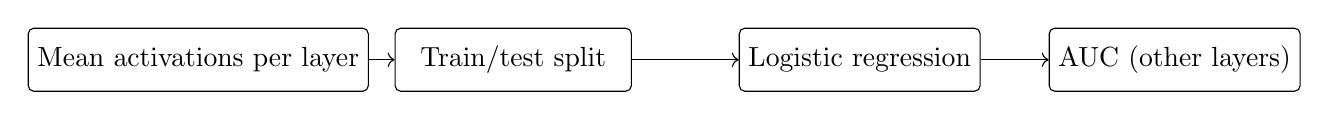
\begin{tikzpicture}[
  node distance=12mm,
  box/.style={draw, rounded corners=2pt, minimum width=30mm, minimum height=8mm, align=center},
  line/.style={->}
]
\node[box] (acts) at (0,0) {Mean activations per layer};
\node[box] (split) at (40mm,0) {Train/test split};
\node[box] (logreg) at (84mm,0) {Logistic regression};
\node[box] (auc) at (124mm,0) {AUC (other layers)};

\draw[line] (acts) -- (split);
\draw[line] (split) -- (logreg);
\draw[line] (logreg) -- (auc);
\end{tikzpicture}
\end{document}

